\section{Complete classification of subcubic six-boundary graphs}\label{sec:subcubic-six}
\begin{theorem}[Six boundary vertices, maximum degree three]\label{thm:subcubic-six}
There are exactly twelve two-connected subcubic graphs with six harmonic
boundary vertices: the ten two-connected subcubic graphs of order six,
the theta graph with path lengths $1,4,4$, and the subdivision of $K_4$
whose three edges in one triangle have length three and whose remaining
three edges have length one. In particular, their maximum order is ten.

Every connected subcubic graph with six harmonic boundary vertices is
obtained by arbitrary independent subdivisions of bridges of exactly one
of 201 reduced kernels. Their maximum order is eighteen, attained by
exactly two kernels. Both consist of four triangles joined by bridges,
with six additional leaves; the four triangle nodes induce $P_4$ or
$K_{1,3}$ in the contracted tree.
\end{theorem}
The new step is an all-orders structural proof for the interior of a
subcubic core. It turns a finite census into an exhaustive classification.
The subsequent block closure is independently certified without orbit
pruning.

\begin{figure}[p]
\centering
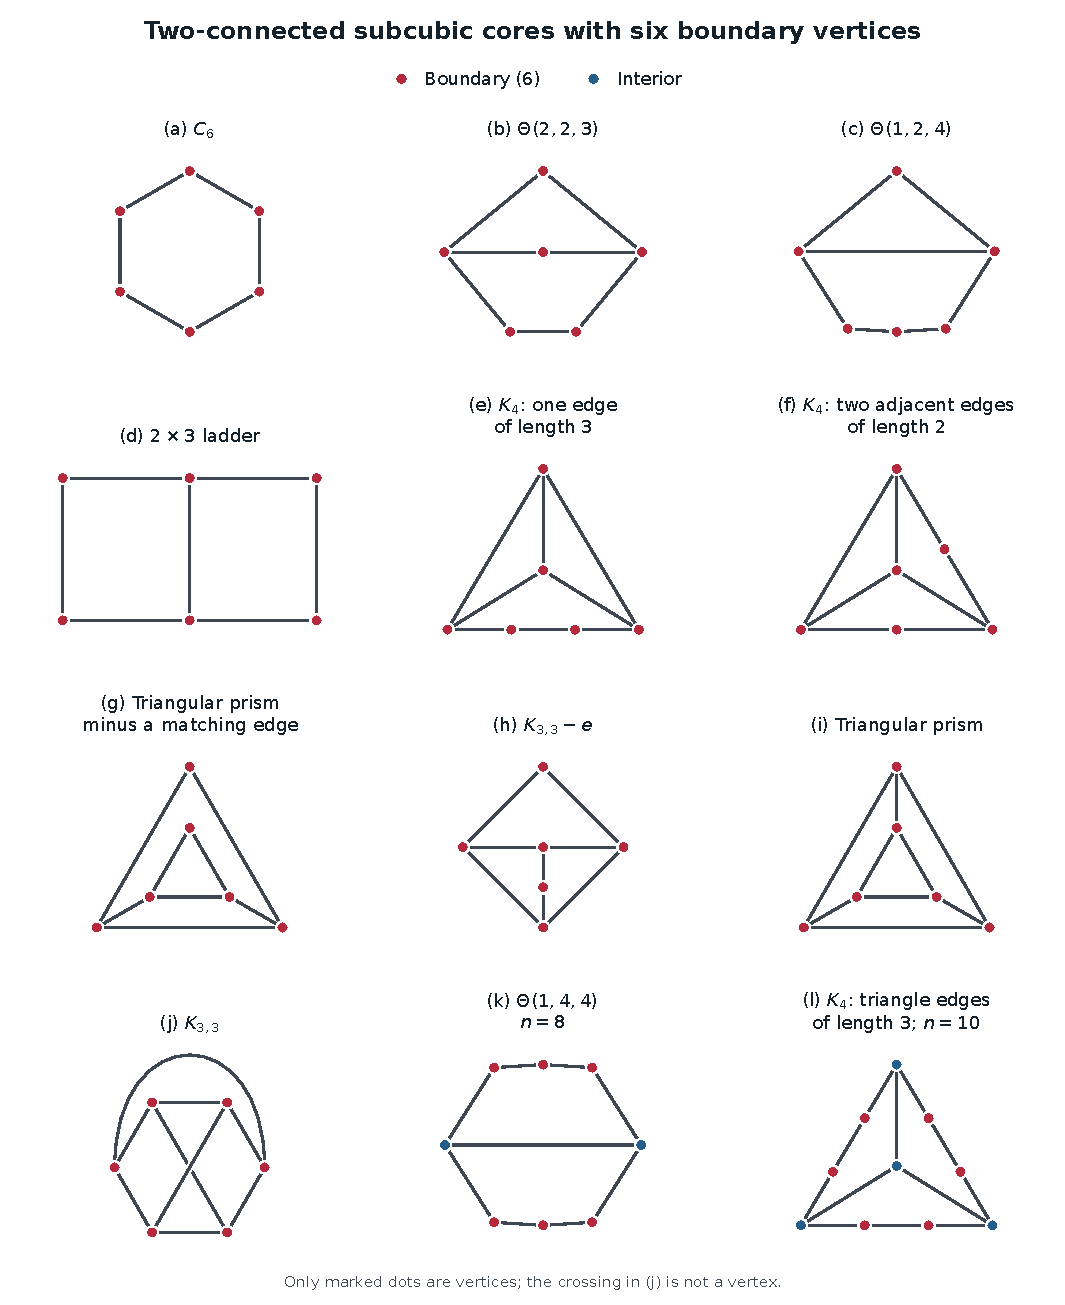
\includegraphics[width=\textwidth,height=.88\textheight,keepaspectratio]{figures/subcubic_twelve_cores.pdf}
\caption{The complete twelve-core subcubic six-boundary palette. The first
ten graphs have order six and all vertices boundary. The last two have
orders eight and ten. Red marks boundary vertices; blue marks interior
vertices. Every model is matched isomorphically to the exact catalogue and
checked by fresh integer shortest-distance calculations.}
\label{fig:subcubic-twelve}
\end{figure}

\subsection{The exact equations at an interior vertex}
Until the block-assembly step, let $G$ be two-connected and subcubic,
$B=\partial G$ with $|B|=6$, $I=V(G)\setminus B$, and $H=G[I]$.
Every vertex of $I$ has degree three in $G$: a degree-two vertex on a
cycle is boundary. The degree-three sector theorem gives independent
neighbors, a unique first neighbor towards each other target, and
exactly two boundary vertices in each of the three first-step sectors.
An edge of $H$ therefore has exactly two boundary coordinates increasing,
two decreasing, and two unchanged.

For a fixed $u\in I$, let its sectors be $S_v$, indexed by its neighbors.
Form a quotient graph $Q_u$ on the three neighbors, putting an edge
between $v,w$ when there is an edge between $S_v,S_w$ in $G-u$.
The quotient is connected. Put
\[
 P_v^w=\{x\in S_v:d(w,x)=d(u,x)\}.
\]
Then $P_v^w$ is nonempty exactly when $vw$ is an edge of $Q_u$.
One direction follows from a horizontal cross-sector edge. For the other,
a shortest $w$--$x$ path of length $r=d(u,x)$ starts at root level one
and ends at level $r$. If $n_-,n_0$ count its inward and horizontal steps,
then $2n_-+n_0=1$. Its sole horizontal step must cross directly from
$S_w$ to $S_v$, since vertical edges preserve sectors.

The sector-flux proof gives a boundary vertex in $P_v^w$ and one in
$S_v\setminus P_v^w$ whenever $P_v^w$ is nonempty. To recall the sign
argument, edges leaving the first set are nonincreasing in distance
from $u$, with at least one strictly decreasing; summing scores cancels
internal edges. For the complement use distance from $w$, with the
strict edge $vu$. Because $S_v$ has exactly two boundary points, precisely
one lies in each set.

If a neighbor $w$ of $u$ is interior, the edge $uw$ has two horizontal
boundary coordinates. Their number equals $\deg_{Q_u}(w)$, so this degree
is two. If a neighbor $v$ is boundary, it belongs to none of the sets
$P_v^w$, since independent root neighbors give $d(w,v)=2$. Quotient
degree two would place its sole sector-mate in both such sets, giving
one closer and two equidistant neighbors at $u$ and hence a positive
score. Thus boundary neighbors have quotient degree one. The connected
quotient is consequently $P_3$ or $K_3$, and
\begin{equation}\label{eq:subcubic-H-degree}
 \deg_H(u)\in\{1,3\}.
\end{equation}
In particular, an $H$ leaf has exactly two boundary neighbors, and an
internal $H$ vertex has none. Also $|I|$ is even.

Let $F(x)=\sum_{b\in B}d(x,b)$. It is constant on each $H$ component.
For an edge from $u\in I$ to $v\in B$, the six changes consist of two
$-1$'s, one zero, and three $+1$'s, so $F(v)=F(u)+1$.
At an internal $H$ vertex, the six nonpositive scores sum to zero.
At an $H$ leaf, their sum is $-2$ and each of its two adjacent boundary
targets gives score $-1$. Hence
\begin{equation}\label{eq:subcubic-exact-score}
 \boxed{\stab_G(u,b)=-\ind_{u\sim b}\qquad(u\in I,\ b\in B).}
\end{equation}
Equivalently, $x\mapsto d(x,b)-\ind_{x=b}$ is harmonic at every interior
vertex. This exact equality is stronger than the defining nonpositive
inequality and is the source of the reduction below.

\subsection{Propagation of tight boundary pairs}
The boundary profiles satisfy
\[
 d(x,y)=\max_{b\in B}|d(x,b)-d(y,b)|,
 \qquad \forall b\ \exists c:\ d(x,b)+d(x,c)=d(b,c).
\]
These properties also follow directly by extending a geodesic away from
its initial target while its endpoint is nonboundary. A nonboundary
endpoint has a farther neighbor, since it has a closer one and nonpositive
score. Strictly increasing distance forces the extension to terminate
at a boundary vertex.

There is no five-cycle in $H$. For each boundary coordinate its horizontal
edges form a matching: two horizontal neighbors would leave one closer
neighbor and give positive score. On a five-cycle the horizontal count is
odd and at most two, hence one. Six coordinates would give six horizontal
edge incidences, while the five edges of $H$ each contribute two, giving
ten. This is impossible.

At an internal $H$ vertex $u$, suppose $b,c$ form a tight pair. Its
nonnegative defect
\[
 g_{bc}(x)=d(x,b)+d(x,c)-d(b,c)
\]
has value zero at $u$. Equation~\eqref{eq:subcubic-exact-score} implies
$\sum_{x\sim u}g_{bc}(x)=0$, so the pair remains tight at every neighbor.
Every coordinate has increments $-1,0,1$ at $u$, and each incident edge is
horizontal in exactly two boundary coordinates. A tight partner must have
the same horizontal edge. Thus the six coordinates are partitioned into
three unique tight pairs. This perfect matching agrees across an edge
between two internal $H$ vertices.

Consider such an edge $uv$, with other neighbors $x,y$ of $u$ and $p,q$
of $v$. On all these vertices, the paired coordinates are complementary.
Select one coordinate from each pair, translate, permute, and reverse
coordinate signs. The exhaustive normal form is
\[
 u=(0,0,0),\quad v=(0,1,1),\quad
 x=(1,0,-1),\quad y=(-1,-1,0),
\]
\[
 p=(\varepsilon,1,2),\quad q=(-\varepsilon,2,1),
 \qquad\varepsilon\in\{-1,1\}.
\]
Both sign cases give $d(y,p)=d(x,q)=2$ by profile isometry.
A common neighbor of $y,p$ cannot be $u,v$ or an interior vertex: the
first choices create a triangle through an interior vertex, and the last
creates a five-cycle $yuvpw$ in $H$. It is therefore boundary. By
\eqref{eq:subcubic-H-degree}, $y,p$ are $H$ leaves. The same holds for $x,q$.
Every internal-to-internal edge therefore exhausts a six-vertex double-star
component. Consequently
\[
 H\text{ has only components }K_2,\ K_{1,3},\text{ or a six-vertex double-star}.
\]
If $\ell$ is its number of leaves, then $|I|\le3\ell/2$ and $|I|$ is even.
Since $2\ell=|E(I,B)|\le18$, this already proves the unconditional
finite bound $|V(G)|\le18$.

\subsection{A sharper hand reduction to order fourteen}
The double-star can in fact be excluded without enumeration. If
$\varepsilon=1$, every selected-coordinate difference between $y,p$ has
absolute value two, as do the complementary differences. A common boundary
neighbor would have distance one from both and hence give a zero difference,
a contradiction.

Suppose $\varepsilon=-1$. Write the actual coordinate values at $u$ as
$D_1,D_2,D_3$ and their complementary values as $D'_1,D'_2,D'_3$.
A boundary neighbor $w$ common to $y,p$, and a boundary neighbor $z$ common
to $x,q$, must be the two endpoints of pair one, forcing
$D_1=D'_1=2$. Positivity on the six interior vertices gives
\[
 D_2,D_3\ge2,\qquad D'_2,D'_3\ge3.
\]
Each $H$ leaf needs a second boundary neighbor. The only coordinate
that can equal one forces respectively
\[
 x\sim c,\quad y\sim a,\quad p\sim c',\quad q\sim a',
 \qquad D_2=D_3=2,\quad D'_2=D'_3=3,
\]
where $(a,a')$ and $(c,c')$ are pairs two and three.
Now $d(x,a)=2$. Among $x$'s neighbors $u,z,c$, the first has distance two
from $a$, and $d(z,a)\ge3$ because $z\sim q$ and $d(q,a)=4$.
Therefore $c\sim a$. The symmetric argument at $p$ forces $c'\sim a'$.
But $d(x,c')=4$, while the distances to $c'$ from $x$'s three neighbors
are $3,5,$ and at most three: the last bound follows from $zqa'c'$.
Thus $\stab_G(x,c')\ge12-(3+5+3)=1$, a contradiction.
We have proved that $H$ has only edge and three-leaf-star components.

There is at most one star component and it precludes every other component.
Its three leaves have distinct boundary neighbors: a shared boundary point
would give two length-two geodesics between interior leaves. Hence its center
has boundary profile $(2,2,2,2,2,2)$. Two centers would violate injectivity.
For a separate edge component $uv$, its four boundary neighbors are distinct.
The two missing boundary coordinates have equal values $r,s$ at $u,v$.
Equation~\eqref{eq:subcubic-exact-score} makes the corresponding distances
from the two boundary neighbors of $u$ equal $r-1,r+1$, and similarly for
$s$. The star center implies that all boundary distances are at most four,
so $r,s\le3$. Every coordinate of $u$ is now between one and three, putting
it at sup-distance at most one from the star center. That would make the
two components adjacent, a contradiction.

Thus either $H=K_{1,3}$ and $|V(G)|=10$, or $H$ is a matching of at most
four edges, because each edge component uses four incidences at the six
boundary vertices. In all cases
\[
 \boxed{|V(G)|\le14.}
\]
An independent standard-library BFS checker exhausts all 60,070
isomorphism classes of two-connected subcubic graphs on orders six through
fourteen, generated by nauty. Exactly twelve have boundary six, and they
are precisely the cores in Theorem~\ref{thm:subcubic-six}. The larger census
through order eighteen, made in the earlier session, is a separate
corroboration. The order bound is proved before either census is used.
The census through order fourteen was repeated without nauty for this
release (Section~\ref{sec:verification}).

\subsection{Exact block assembly and the 201 kernels}
At intrinsic boundary at most five, every two-connected subcubic block is
all boundary, by the degree-three obstruction. Its order is at most five.
The full palette therefore consists of all two-connected subcubic graphs
on three through six vertices, and the exceptional cores of orders eight
and ten: twenty nonbridge types in total.

Distinct nonbridge blocks of a subcubic graph are vertex-disjoint. Bridges
attach only at intrinsic degree-two block vertices, at most one per vertex.
At such a vertex the intrinsic stability is one or two; one external bridge
lowers it by one. Let $h_C$ count attached sites of intrinsic stability one,
and let $L$ count ordinary leaves outside the blocks. The exact assembly
condition is
\begin{equation}\label{eq:subcubic-six-assembly}
 6=L+\sum_C\bigl(b(C)-h_C\bigr).
\end{equation}
Choose any block tree from the palette, with ordinary vertices of degrees
one or three, attach its bridges injectively to available degree-two sites,
and impose \eqref{eq:subcubic-six-assembly}. Together with arbitrary bridge
subdivision, this is a necessary-and-sufficient constructive description.

For the reduced-order bound, write $R=\sum_C(b(C)-2)$ and let $\Delta_*\ge0$
be the total cut defect in the exact block budget. Then $R+\Delta_*=4$.
Every palette block satisfies $|V(C)|\le3(b(C)-2)$, with equality only for
a triangle. If $A$ counts ordinary degree-three vertices, each contributes
at least one cut defect, so $A\le\Delta_*$. Since $L\le6$,
\[
 |V(K)|=\sum_C|V(C)|+A+L
 \le3R+\Delta_*+6=18-2\Delta_*\le18.
\]
Equality forces four triangles, six ordinary leaves, no ordinary branch
vertex, and every triangle site buried by a bridge. The contracted tree
has four trivalent internal nodes, whose induced tree is $P_4$ or
$K_{1,3}$. These give exactly the two equality kernels.

\begin{figure}[p]
\centering
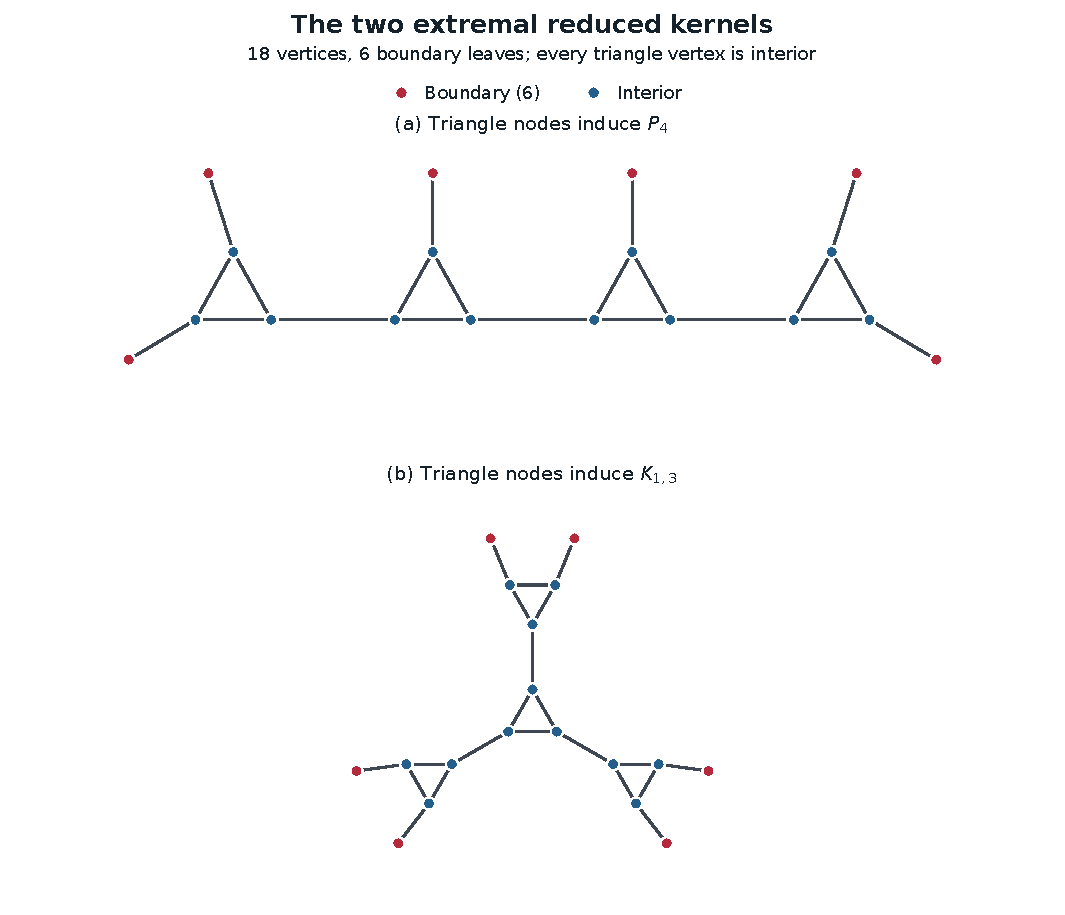
\includegraphics[width=\textwidth]{figures/subcubic_extremizers18.pdf}
\caption{The two eighteen-vertex reduced kernels attaining the sharp
subcubic six-boundary bound. Their boundary consists of the six leaves.
Arbitrary subdivisions of the displayed bridges preserve the boundary.}
\label{fig:subcubic-extremizers}
\end{figure}

The finite closure uses rooted block attachment and insertion of a new
trivalent branch on a bridge, retaining maximum degree three and boundary
at most six. The usual end-block induction proves completeness. There
are 264 states of boundary at most six, of which 201 have boundary six.
Their order distribution is
\begin{center}\small
\begin{tabular}{@{}rrrrrrrrrrrrrr@{}}\toprule
$n$&6&7&8&9&10&11&12&13&14&15&16&17&18\\\midrule
Number&16&8&10&9&23&20&32&25&27&15&11&3&2\\\bottomrule
\end{tabular}
\end{center}
The independent verifier imports no generator and uses no orbit pruning.
It checks all 47,332 degree-admissible vertex/root attachments, all 1,257
bridge branchings, fresh boundary scores and reducedness for every state,
well-founded generation of every nonseed, and exact canonical closure.
The 63 states with boundary at most five agree exactly with the previous
subcubic catalogue. The whole subcubic six-boundary proof is not claimed
to be formalized in Lean; its sector input is formalized, its new reductions
are conventional proofs, and its finite catalogues have exact
reproducible checkers.
